\documentclass{standalone}
\usepackage{tikz}
\usetikzlibrary{patterns, positioning}


\begin{document}
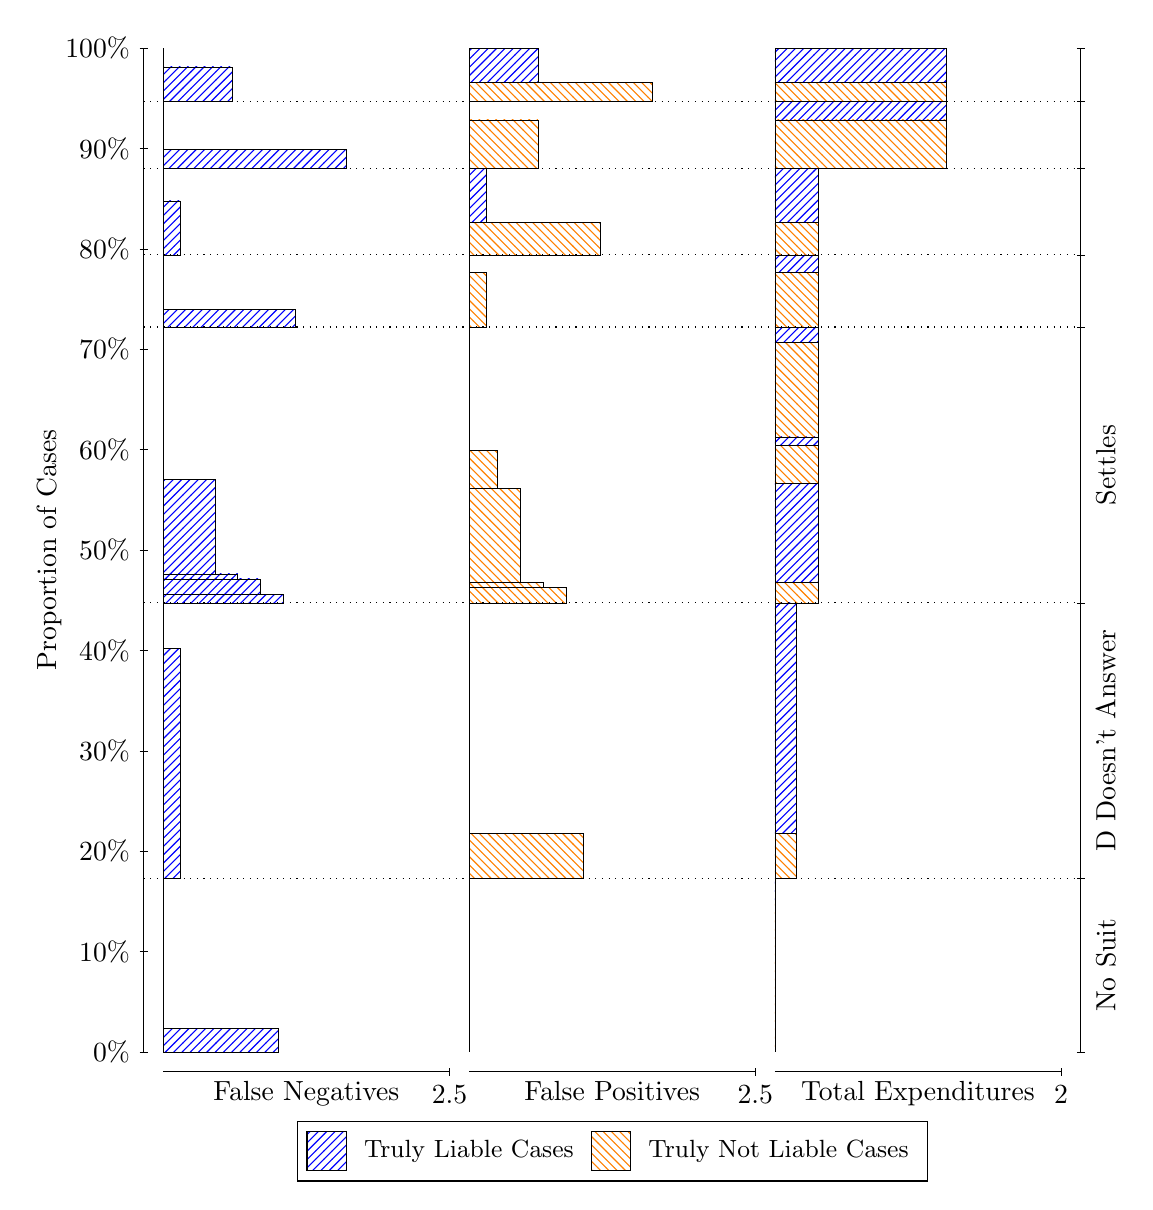
\begin{tikzpicture}
\draw[black, very thin] (1.5,1.75) -- (1.5,14.5);
\node[rotate=90, text=black, anchor=center] at (0.3, 8.125) {Proportion of Cases};
\draw[black, very thin] (1.45,1.75) -- (1.55,1.75);
\node[text=black, anchor=east] at (1.45, 1.75) {0\%};
\draw[black, very thin] (1.45,3.025) -- (1.55,3.025);
\node[text=black, anchor=east] at (1.45, 3.025) {10\%};
\draw[black, very thin] (1.45,4.3) -- (1.55,4.3);
\node[text=black, anchor=east] at (1.45, 4.3) {20\%};
\draw[black, very thin] (1.45,5.575) -- (1.55,5.575);
\node[text=black, anchor=east] at (1.45, 5.575) {30\%};
\draw[black, very thin] (1.45,6.85) -- (1.55,6.85);
\node[text=black, anchor=east] at (1.45, 6.85) {40\%};
\draw[black, very thin] (1.45,8.125) -- (1.55,8.125);
\node[text=black, anchor=east] at (1.45, 8.125) {50\%};
\draw[black, very thin] (1.45,9.4) -- (1.55,9.4);
\node[text=black, anchor=east] at (1.45, 9.4) {60\%};
\draw[black, very thin] (1.45,10.675) -- (1.55,10.675);
\node[text=black, anchor=east] at (1.45, 10.675) {70\%};
\draw[black, very thin] (1.45,11.95) -- (1.55,11.95);
\node[text=black, anchor=east] at (1.45, 11.95) {80\%};
\draw[black, very thin] (1.45,13.225) -- (1.55,13.225);
\node[text=black, anchor=east] at (1.45, 13.225) {90\%};
\draw[black, very thin] (1.45,14.5) -- (1.55,14.5);
\node[text=black, anchor=east] at (1.45, 14.5) {100\%};

\draw[black, very thin] (13.4,1.75) -- (13.4,14.5);
\draw[black, very thin] (13.35,1.75) -- (13.45,1.75);
\node[anchor=west] at (13.35, 1.75) {};
\draw[black, very thin] (13.35,3.9523) -- (13.45,3.9523);
\node[anchor=west] at (13.35, 3.9523) {};
\draw[black, very thin] (13.35,7.4532) -- (13.45,7.4532);
\node[anchor=west] at (13.35, 7.4532) {};
\draw[black, very thin] (13.35,10.957) -- (13.45,10.957);
\node[anchor=west] at (13.35, 10.957) {};
\draw[black, very thin] (13.35,11.873) -- (13.45,11.873);
\node[anchor=west] at (13.35, 11.873) {};
\draw[black, very thin] (13.35,12.971) -- (13.45,12.971);
\node[anchor=west] at (13.35, 12.971) {};
\draw[black, very thin] (13.35,13.826) -- (13.45,13.826);
\node[anchor=west] at (13.35, 13.826) {};
\draw[black, very thin] (13.35,14.5) -- (13.45,14.5);
\node[anchor=west] at (13.35, 14.5) {};

\draw[black, very thin, pattern color=blue, pattern=north east lines] (1.75,1.75) rectangle (3.2033,2.0497);
\draw[black, very thin, pattern color=orange, pattern=north west lines] (1.75,2.0497) rectangle (1.75,3.9523);
\draw[black, very thin, pattern color=blue, pattern=north east lines] (1.75,3.9523) rectangle (1.968,6.8775);
\draw[black, very thin, pattern color=orange, pattern=north west lines] (1.75,6.8775) rectangle (1.75,7.4532);
\draw[black, very thin, pattern color=blue, pattern=north east lines] (1.75,7.4532) rectangle (3.276,7.5592);
\draw[black, very thin, pattern color=blue, pattern=north east lines] (1.75,7.5592) rectangle (2.9853,7.7577);
\draw[black, very thin, pattern color=blue, pattern=north east lines] (1.75,7.7577) rectangle (2.6947,7.8203);
\draw[black, very thin, pattern color=blue, pattern=north east lines] (1.75,7.8203) rectangle (2.404,9.0182);
\draw[black, very thin, pattern color=orange, pattern=north west lines] (1.75,9.0182) rectangle (1.75,10.957);
\draw[black, very thin, pattern color=blue, pattern=north east lines] (1.75,10.957) rectangle (3.4213,11.183);
\draw[black, very thin, pattern color=orange, pattern=north west lines] (1.75,11.183) rectangle (1.75,11.873);
\draw[black, very thin, pattern color=blue, pattern=north east lines] (1.75,11.873) rectangle (1.968,12.559);
\draw[black, very thin, pattern color=orange, pattern=north west lines] (1.75,12.559) rectangle (1.75,12.971);
\draw[black, very thin, pattern color=blue, pattern=north east lines] (1.75,12.971) rectangle (4.0753,13.21);
\draw[black, very thin, pattern color=orange, pattern=north west lines] (1.75,13.21) rectangle (1.75,13.826);
\draw[black, very thin, pattern color=blue, pattern=north east lines] (1.75,13.826) rectangle (2.622,14.261);
\draw[black, very thin, pattern color=orange, pattern=north west lines] (1.75,14.261) rectangle (1.75,14.5);
\draw[black, very thin, pattern color=orange, pattern=north west lines] (5.6333,1.75) rectangle (5.6333,3.6526);
\draw[black, very thin, pattern color=blue, pattern=north east lines] (5.6333,3.6526) rectangle (5.6333,3.9523);
\draw[black, very thin, pattern color=orange, pattern=north west lines] (5.6333,3.9523) rectangle (7.0867,4.528);
\draw[black, very thin, pattern color=blue, pattern=north east lines] (5.6333,4.528) rectangle (5.6333,7.4532);
\draw[black, very thin, pattern color=orange, pattern=north west lines] (5.6333,7.4532) rectangle (6.8687,7.6517);
\draw[black, very thin, pattern color=orange, pattern=north west lines] (5.6333,7.6517) rectangle (6.578,7.7142);
\draw[black, very thin, pattern color=orange, pattern=north west lines] (5.6333,7.7142) rectangle (6.2873,8.9122);
\draw[black, very thin, pattern color=orange, pattern=north west lines] (5.6333,8.9122) rectangle (5.9967,9.3923);
\draw[black, very thin, pattern color=blue, pattern=north east lines] (5.6333,9.3923) rectangle (5.6333,10.957);
\draw[black, very thin, pattern color=orange, pattern=north west lines] (5.6333,10.957) rectangle (5.8513,11.648);
\draw[black, very thin, pattern color=blue, pattern=north east lines] (5.6333,11.648) rectangle (5.6333,11.873);
\draw[black, very thin, pattern color=orange, pattern=north west lines] (5.6333,11.873) rectangle (7.3047,12.285);
\draw[black, very thin, pattern color=blue, pattern=north east lines] (5.6333,12.285) rectangle (5.8513,12.971);
\draw[black, very thin, pattern color=orange, pattern=north west lines] (5.6333,12.971) rectangle (6.5053,13.587);
\draw[black, very thin, pattern color=blue, pattern=north east lines] (5.6333,13.587) rectangle (5.6333,13.826);
\draw[black, very thin, pattern color=orange, pattern=north west lines] (5.6333,13.826) rectangle (7.9587,14.065);
\draw[black, very thin, pattern color=blue, pattern=north east lines] (5.6333,14.065) rectangle (6.5053,14.5);
\draw[black, very thin, pattern color=orange, pattern=north west lines] (9.5167,1.75) rectangle (9.5167,3.6526);
\draw[black, very thin, pattern color=blue, pattern=north east lines] (9.5167,3.6526) rectangle (9.5167,3.9523);
\draw[black, very thin, pattern color=orange, pattern=north west lines] (9.5167,3.9523) rectangle (9.7892,4.528);
\draw[black, very thin, pattern color=blue, pattern=north east lines] (9.5167,4.528) rectangle (9.7892,7.4532);
\draw[black, very thin, pattern color=orange, pattern=north west lines] (9.5167,7.4532) rectangle (10.062,7.7142);
\draw[black, very thin, pattern color=blue, pattern=north east lines] (9.5167,7.7142) rectangle (10.062,8.9747);
\draw[black, very thin, pattern color=orange, pattern=north west lines] (9.5167,8.9747) rectangle (10.062,9.4548);
\draw[black, very thin, pattern color=blue, pattern=north east lines] (9.5167,9.4548) rectangle (10.062,9.5608);
\draw[black, very thin, pattern color=orange, pattern=north west lines] (9.5167,9.5608) rectangle (10.062,10.759);
\draw[black, very thin, pattern color=blue, pattern=north east lines] (9.5167,10.759) rectangle (10.062,10.957);
\draw[black, very thin, pattern color=orange, pattern=north west lines] (9.5167,10.957) rectangle (10.062,11.648);
\draw[black, very thin, pattern color=blue, pattern=north east lines] (9.5167,11.648) rectangle (10.062,11.873);
\draw[black, very thin, pattern color=orange, pattern=north west lines] (9.5167,11.873) rectangle (10.062,12.285);
\draw[black, very thin, pattern color=blue, pattern=north east lines] (9.5167,12.285) rectangle (10.062,12.971);
\draw[black, very thin, pattern color=orange, pattern=north west lines] (9.5167,12.971) rectangle (11.697,13.587);
\draw[black, very thin, pattern color=blue, pattern=north east lines] (9.5167,13.587) rectangle (11.697,13.826);
\draw[black, very thin, pattern color=orange, pattern=north west lines] (9.5167,13.826) rectangle (11.697,14.065);
\draw[black, very thin, pattern color=blue, pattern=north east lines] (9.5167,14.065) rectangle (11.697,14.5);
\draw[black, dotted] (1.5,3.9523) -- (13.4,3.9523);
\draw[black, dotted] (1.5,7.4532) -- (13.4,7.4532);
\draw[black, dotted] (1.5,10.957) -- (13.4,10.957);
\draw[black, dotted] (1.5,11.873) -- (13.4,11.873);
\draw[black, dotted] (1.5,12.971) -- (13.4,12.971);
\draw[black, dotted] (1.5,13.826) -- (13.4,13.826);
\draw[black, very thin] (1.75,1.5) -- (5.3833,1.5);
\node[text=black, anchor=north] at (3.5667, 1.5) {False Negatives};
\draw[black, very thin] (5.3833,1.45) -- (5.3833,1.55);
\node[text=black, anchor=north] at (5.3833, 1.45) {2.5};

\draw[black, very thin] (5.6333,1.5) -- (9.2667,1.5);
\node[text=black, anchor=north] at (7.45, 1.5) {False Positives};
\draw[black, very thin] (9.2667,1.45) -- (9.2667,1.55);
\node[text=black, anchor=north] at (9.2667, 1.45) {2.5};

\draw[black, very thin] (9.5167,1.5) -- (13.15,1.5);
\node[text=black, anchor=north] at (11.333, 1.5) {Total Expenditures};
\draw[black, very thin] (13.15,1.45) -- (13.15,1.55);
\node[text=black, anchor=north] at (13.15, 1.45) {2};

\node[text=black, centered, rotate=90] at (13.72, 2.8511) {No Suit};
\node[text=black, centered, rotate=90] at (13.72, 5.7027) {D Doesn't Answer};
\node[text=black, centered, rotate=90] at (13.72, 9.2052) {Settles};





\draw (7.449999999999999,1.5) node[draw=none] (baseCoordinate) {};
\begin{scope}[align=center]
        \matrix[scale=0.5, draw=black, below=0.5cm of baseCoordinate, nodes={draw}, column sep=0.1cm]{
            \node[rectangle, draw, minimum width=0.5cm, minimum height=0.5cm, pattern color=blue, pattern=north east lines] {}; &
            \node[draw=none, font=\small, text=black] (B) {Truly Liable Cases}; &
            \node[rectangle, draw, minimum width=0.5cm, minimum height=0.5cm, pattern color=orange, pattern=north west lines] {}; &
            \node[draw=none, font=\small, text=black] (B) {Truly Not Liable Cases}; \\
            };
\end{scope}

\end{tikzpicture}
\end{document}